\PassOptionsToPackage{unicode=true}{hyperref} % options for packages loaded elsewhere
\PassOptionsToPackage{hyphens}{url}
%
\documentclass[]{article}
\usepackage{lmodern}
\usepackage{amssymb,amsmath}
\usepackage{ifxetex,ifluatex}
\usepackage{fixltx2e} % provides \textsubscript
\ifnum 0\ifxetex 1\fi\ifluatex 1\fi=0 % if pdftex
  \usepackage[T1]{fontenc}
  \usepackage[utf8]{inputenc}
  \usepackage{textcomp} % provides euro and other symbols
\else % if luatex or xelatex
  \usepackage{unicode-math}
  \defaultfontfeatures{Ligatures=TeX,Scale=MatchLowercase}
\fi
% use upquote if available, for straight quotes in verbatim environments
\IfFileExists{upquote.sty}{\usepackage{upquote}}{}
% use microtype if available
\IfFileExists{microtype.sty}{%
\usepackage[]{microtype}
\UseMicrotypeSet[protrusion]{basicmath} % disable protrusion for tt fonts
}{}
\IfFileExists{parskip.sty}{%
\usepackage{parskip}
}{% else
\setlength{\parindent}{0pt}
\setlength{\parskip}{6pt plus 2pt minus 1pt}
}
\usepackage{hyperref}
\hypersetup{
            pdftitle={Project3},
            pdfauthor={Rongkui Han},
            pdfborder={0 0 0},
            breaklinks=true}
\urlstyle{same}  % don't use monospace font for urls
\usepackage[margin=1in]{geometry}
\usepackage{color}
\usepackage{fancyvrb}
\newcommand{\VerbBar}{|}
\newcommand{\VERB}{\Verb[commandchars=\\\{\}]}
\DefineVerbatimEnvironment{Highlighting}{Verbatim}{commandchars=\\\{\}}
% Add ',fontsize=\small' for more characters per line
\usepackage{framed}
\definecolor{shadecolor}{RGB}{248,248,248}
\newenvironment{Shaded}{\begin{snugshade}}{\end{snugshade}}
\newcommand{\AlertTok}[1]{\textcolor[rgb]{0.94,0.16,0.16}{#1}}
\newcommand{\AnnotationTok}[1]{\textcolor[rgb]{0.56,0.35,0.01}{\textbf{\textit{#1}}}}
\newcommand{\AttributeTok}[1]{\textcolor[rgb]{0.77,0.63,0.00}{#1}}
\newcommand{\BaseNTok}[1]{\textcolor[rgb]{0.00,0.00,0.81}{#1}}
\newcommand{\BuiltInTok}[1]{#1}
\newcommand{\CharTok}[1]{\textcolor[rgb]{0.31,0.60,0.02}{#1}}
\newcommand{\CommentTok}[1]{\textcolor[rgb]{0.56,0.35,0.01}{\textit{#1}}}
\newcommand{\CommentVarTok}[1]{\textcolor[rgb]{0.56,0.35,0.01}{\textbf{\textit{#1}}}}
\newcommand{\ConstantTok}[1]{\textcolor[rgb]{0.00,0.00,0.00}{#1}}
\newcommand{\ControlFlowTok}[1]{\textcolor[rgb]{0.13,0.29,0.53}{\textbf{#1}}}
\newcommand{\DataTypeTok}[1]{\textcolor[rgb]{0.13,0.29,0.53}{#1}}
\newcommand{\DecValTok}[1]{\textcolor[rgb]{0.00,0.00,0.81}{#1}}
\newcommand{\DocumentationTok}[1]{\textcolor[rgb]{0.56,0.35,0.01}{\textbf{\textit{#1}}}}
\newcommand{\ErrorTok}[1]{\textcolor[rgb]{0.64,0.00,0.00}{\textbf{#1}}}
\newcommand{\ExtensionTok}[1]{#1}
\newcommand{\FloatTok}[1]{\textcolor[rgb]{0.00,0.00,0.81}{#1}}
\newcommand{\FunctionTok}[1]{\textcolor[rgb]{0.00,0.00,0.00}{#1}}
\newcommand{\ImportTok}[1]{#1}
\newcommand{\InformationTok}[1]{\textcolor[rgb]{0.56,0.35,0.01}{\textbf{\textit{#1}}}}
\newcommand{\KeywordTok}[1]{\textcolor[rgb]{0.13,0.29,0.53}{\textbf{#1}}}
\newcommand{\NormalTok}[1]{#1}
\newcommand{\OperatorTok}[1]{\textcolor[rgb]{0.81,0.36,0.00}{\textbf{#1}}}
\newcommand{\OtherTok}[1]{\textcolor[rgb]{0.56,0.35,0.01}{#1}}
\newcommand{\PreprocessorTok}[1]{\textcolor[rgb]{0.56,0.35,0.01}{\textit{#1}}}
\newcommand{\RegionMarkerTok}[1]{#1}
\newcommand{\SpecialCharTok}[1]{\textcolor[rgb]{0.00,0.00,0.00}{#1}}
\newcommand{\SpecialStringTok}[1]{\textcolor[rgb]{0.31,0.60,0.02}{#1}}
\newcommand{\StringTok}[1]{\textcolor[rgb]{0.31,0.60,0.02}{#1}}
\newcommand{\VariableTok}[1]{\textcolor[rgb]{0.00,0.00,0.00}{#1}}
\newcommand{\VerbatimStringTok}[1]{\textcolor[rgb]{0.31,0.60,0.02}{#1}}
\newcommand{\WarningTok}[1]{\textcolor[rgb]{0.56,0.35,0.01}{\textbf{\textit{#1}}}}
\usepackage{longtable,booktabs}
% Fix footnotes in tables (requires footnote package)
\IfFileExists{footnote.sty}{\usepackage{footnote}\makesavenoteenv{longtable}}{}
\usepackage{graphicx,grffile}
\makeatletter
\def\maxwidth{\ifdim\Gin@nat@width>\linewidth\linewidth\else\Gin@nat@width\fi}
\def\maxheight{\ifdim\Gin@nat@height>\textheight\textheight\else\Gin@nat@height\fi}
\makeatother
% Scale images if necessary, so that they will not overflow the page
% margins by default, and it is still possible to overwrite the defaults
% using explicit options in \includegraphics[width, height, ...]{}
\setkeys{Gin}{width=\maxwidth,height=\maxheight,keepaspectratio}
\setlength{\emergencystretch}{3em}  % prevent overfull lines
\providecommand{\tightlist}{%
  \setlength{\itemsep}{0pt}\setlength{\parskip}{0pt}}
\setcounter{secnumdepth}{5}
% Redefines (sub)paragraphs to behave more like sections
\ifx\paragraph\undefined\else
\let\oldparagraph\paragraph
\renewcommand{\paragraph}[1]{\oldparagraph{#1}\mbox{}}
\fi
\ifx\subparagraph\undefined\else
\let\oldsubparagraph\subparagraph
\renewcommand{\subparagraph}[1]{\oldsubparagraph{#1}\mbox{}}
\fi

% set default figure placement to htbp
\makeatletter
\def\fps@figure{htbp}
\makeatother


\title{Project3}
\author{Rongkui Han}
\date{2/6/2020}

\begin{document}
\maketitle

\hypertarget{examining-covariate-balance-in-the-matched-sample}{%
\subsection{Examining covariate balance in the matched sample}\label{examining-covariate-balance-in-the-matched-sample}}

We'll do three things to assess covariate balance in the matched sample:

\begin{itemize}
\tightlist
\item
  visual inspection
\item
  t-tests of difference-in-means
\item
  computation of the average absolute standardized difference (``standardized imbalance'')
\end{itemize}

\begin{Shaded}
\begin{Highlighting}[]
\NormalTok{fn_bal <-}\StringTok{ }\ControlFlowTok{function}\NormalTok{(dta, variable) \{}
\NormalTok{  dta}\OperatorTok{$}\NormalTok{variable <-}\StringTok{ }\NormalTok{dta[, variable]}
\NormalTok{  dta}\OperatorTok{$}\NormalTok{jail <-}\StringTok{ }\KeywordTok{as.factor}\NormalTok{(dta}\OperatorTok{$}\NormalTok{jail)}
\NormalTok{  support <-}\StringTok{ }\KeywordTok{c}\NormalTok{(}\KeywordTok{min}\NormalTok{(dta}\OperatorTok{$}\NormalTok{variable), }\KeywordTok{max}\NormalTok{(dta}\OperatorTok{$}\NormalTok{variable))}
  \KeywordTok{ggplot}\NormalTok{(dta, }\KeywordTok{aes}\NormalTok{(}\DataTypeTok{x =}\NormalTok{ distance, }\DataTypeTok{y =}\NormalTok{ variable, }\DataTypeTok{color =}\NormalTok{ jail)) }\OperatorTok{+}
\StringTok{    }\KeywordTok{geom_point}\NormalTok{(}\DataTypeTok{alpha =} \FloatTok{0.2}\NormalTok{, }\DataTypeTok{size =} \FloatTok{1.3}\NormalTok{) }\OperatorTok{+}
\StringTok{    }\KeywordTok{geom_smooth}\NormalTok{(}\DataTypeTok{method =} \StringTok{"loess"}\NormalTok{, }\DataTypeTok{se =}\NormalTok{ F) }\OperatorTok{+}
\StringTok{    }\KeywordTok{xlab}\NormalTok{(}\StringTok{"Propensity score"}\NormalTok{) }\OperatorTok{+}
\StringTok{    }\KeywordTok{ylab}\NormalTok{(variable) }\OperatorTok{+}
\StringTok{    }\KeywordTok{theme_bw}\NormalTok{() }\OperatorTok{+}
\StringTok{    }\KeywordTok{ylim}\NormalTok{(support)}
\NormalTok{\}}

\KeywordTok{grid.arrange}\NormalTok{(}
   \CommentTok{#fn_bal(dta_m, "year"),}
   \KeywordTok{fn_bal}\NormalTok{(dta_m, }\StringTok{"spirits"}\NormalTok{),}
   \KeywordTok{fn_bal}\NormalTok{(dta_m, }\StringTok{"unemp"}\NormalTok{),}
   \KeywordTok{fn_bal}\NormalTok{(dta_m, }\StringTok{"income"}\NormalTok{), }\CommentTok{#+ theme(legend.position = "none"),}
   \KeywordTok{fn_bal}\NormalTok{(dta_m, }\StringTok{"beertax"}\NormalTok{),}
   \CommentTok{#fn_bal(dta_m, "baptist"),}
   \CommentTok{#fn_bal(dta_m, "mormon"),}
   \KeywordTok{fn_bal}\NormalTok{(dta_m, }\StringTok{"drinkage"}\NormalTok{),}
   \KeywordTok{fn_bal}\NormalTok{(dta_m, }\StringTok{"dry"}\NormalTok{),}
   \KeywordTok{fn_bal}\NormalTok{(dta_m, }\StringTok{"youngdrivers"}\NormalTok{),}
   \KeywordTok{fn_bal}\NormalTok{(dta_m, }\StringTok{"miles"}\NormalTok{),}
   \CommentTok{#fn_bal(dta_m, "breath"),}
   \KeywordTok{fn_bal}\NormalTok{(dta_m, }\StringTok{"pop"}\NormalTok{),}
   \KeywordTok{fn_bal}\NormalTok{(dta_m, }\StringTok{"gsp"}\NormalTok{),}
   \DataTypeTok{nrow =} \DecValTok{4}\CommentTok{#, widths = c(1, 0.8)}
\NormalTok{)}
\end{Highlighting}
\end{Shaded}

\begin{verbatim}
## Warning: Removed 19 rows containing missing values (geom_smooth).
\end{verbatim}

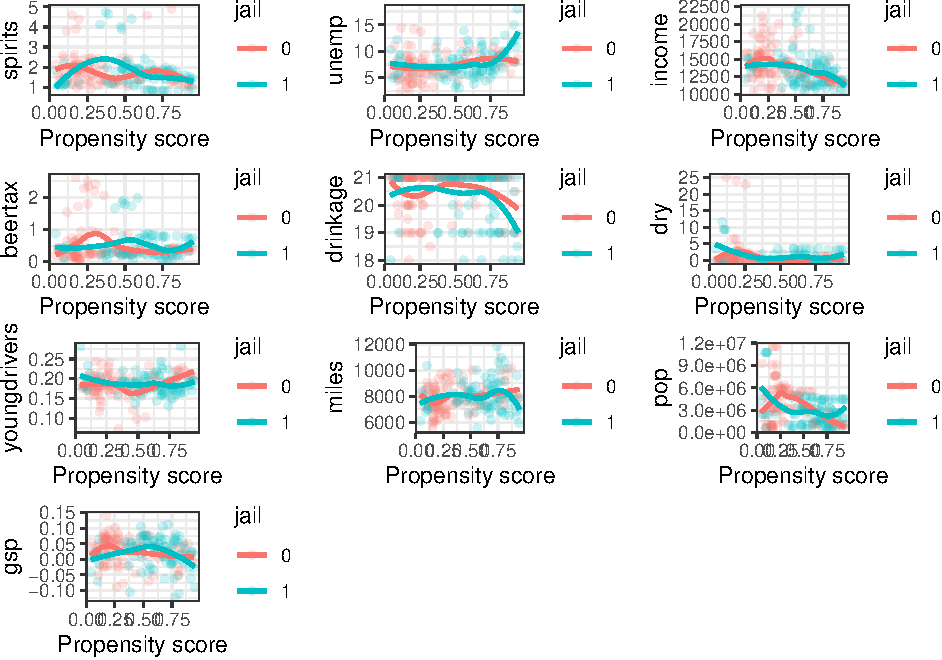
\includegraphics{Project3_Rongkui_files/figure-latex/unnamed-chunk-8-1.pdf}

\begin{center}\rule{0.5\linewidth}{0.5pt}\end{center}

\hypertarget{team-id-team-6}{%
\subsubsection{Team ID: Team 6}\label{team-id-team-6}}

\hypertarget{name-connor-rosenberg}{%
\paragraph{NAME: Connor Rosenberg}\label{name-connor-rosenberg}}

\hypertarget{name-rongkui-han}{%
\paragraph{NAME: Rongkui Han}\label{name-rongkui-han}}

\hypertarget{name-yuqing-yang}{%
\paragraph{NAME: Yuqing Yang}\label{name-yuqing-yang}}

\hypertarget{name-nassim-ali-chaouche}{%
\paragraph{NAME: Nassim Ali-Chaouche}\label{name-nassim-ali-chaouche}}

\begin{center}\rule{0.5\linewidth}{0.5pt}\end{center}

\hypertarget{introduction}{%
\subsection{1.0 Introduction}\label{introduction}}

\hypertarget{background}{%
\paragraph{1.1 Background}\label{background}}

Traffic accidents cause thousands of deaths in the United States every year. Data pertinent to US traffic fatalities from the years 1982 to 1988 can be easily accessed in the ``Fatalities'' dataset. The data was obtained from sources such as the US Department of Transportation Fatal Accident Reporting System (FARS) and the US Bureau of Labor Statistics. The dataset includes panel data for 48 states (Alaska and Hawaii not included), containing demographic variables such as population, income per capita, religious belief, and unemployment rate. In addition, features that are commonly associated with traffic accidents and its regulation, such as average miles per driver, percentage of young drivers, tax collected per case of beer, presence of a preliminary breath test law, and whether the state implemented mandatory jail sentences or community service for an initial drunk driving conviction, were also presented in the dataset. Finally, the number of vehicle fatalities and its numerous subsets, such as night-time or single-vehicle fatalities, were introduced. The observations were recorded for each state annually. In total, there are 336 observations recorded for 34 distinct variables.

Due to the observational nature of the data, obtaining causal effects may pose a challenge. In observational studies, treatment selection is often influenced by subject characteristics. In the context of our study, ``treatment assignment'' refers to whether a state has a mandatory jail sentence for an initial drunk driving conviction. It is not difficult to imagine that demographic characteristics of a state can influence both its traffic legislations as well as its traffic fatality rate, causing confounding effects that obscure the impact of legislation on traffic fatality. As a result, systematic differences in baseline characteristics between states with and without mandatory jail sentences must be taken into account when estimating its effect on outcomes. The \textbf{propensity score} is the probability of treatment assignment conditional on observed baseline characteristics. The propensity score allows one to analyze an observational study so that it mimics some of the particular characteristics of a randomized controlled trial. In particular, conditional on the propensity score, the distribution of observed baseline covariates will be similar between treated and untreated subjects, allowing the estimation of the average treatment effect (Austin, 2011). In this report, we will attempt to discover the potential causal relationship between a mandatory jail sentence for an initial drunk driving conviction and the traffic fatality rate of the state using the \textbf{propensity score matching} technique, followed by \textbf{mixed-effect ANOVA modeling}. The primary objective of this analysis is to educate State legislators on whether a mandatory jail sentence is a proper current and will result in lower automobile fatality rates.

\hypertarget{questions-of-interest}{%
\paragraph{1.2 Questions of Interest}\label{questions-of-interest}}

\begin{itemize}
\tightlist
\item
  Are there demographic features that correlate with a state's mandatory jail sentence law?\\
\item
  Is a state's mandatory jail sentence law associated with its annual traffic fatality rate, without adjusting for potential covariating demographic variables?\\
\item
  Is a state's mandatory jail sentence law associated with its annual traffic fatality rate, after adjusting for potential covariating demographic variables?\\
\item
  Can we draw a causal conclusion regarding the relationship between a state's mandatory jail sentence law and its annual traffic fatality rate?
\end{itemize}

\hypertarget{analysis-plan}{%
\subsection{2.0 Analysis Plan}\label{analysis-plan}}

From data collected by the National Highway Traffic Safety Administration's FARS, we plan to conduct a propensity score analysis followed by mixed-effect ANOVA modeling to isolate the average effect of required jail time on automobile fatality rates.

\hypertarget{population-and-study-design}{%
\paragraph{2.1 Population and study design}\label{population-and-study-design}}

The response variable used in this analysis is the yearly traffic fatality rate per 10,000 population. This statistic will be calculated by dividing a state's total traffic fatality count within a given year by its population of the year, multiplied by 10,000.

The ``Fatalities'' dataset is a longitudinal dataset, also know as ``panel dataset'', with a ``year'' index that delineates the temporal order of entries. In a typical panel dataset, each individual has multiple entries, some of which correspond to pre-treatment records while others post-treatment. In this regard, the vehicle fatality dataset is atypical, because only six out of 48 states had pre- and post-treatment records (\emph{Figure X}). Most states did not change their mandatory jail sentence policy between 1982 and 1988. Due to this limitation, common panel data analysis techniques are not applicable. In response, we will follow a bench-marked pipeline for analyzing non-panel observational data under a propensity score matching framework (Smith, 1997), while closely monitoring the behavior of the temperal variable throughout the analysis, and address any potential issues that might arise.

\hypertarget{descriptive-analysis}{%
\paragraph{2.2 Descriptive Analysis}\label{descriptive-analysis}}

\hypertarget{propensity-score-analysis}{%
\paragraph{2.3 Propensity Score Analysis}\label{propensity-score-analysis}}

\hypertarget{propensity-score-estimation}{%
\subparagraph{2.3.1 Propensity Score Estimation}\label{propensity-score-estimation}}

We will estimate the propensity score through a logistic regression model. The dependent variable of the logistic regression model is a binary variable indicating treatment status, whether or not a State has a mandatory jail sentence. There is a lack of consensus in the applied literature as to which variables to include in the propensity score model (Austin, 2001). Brookhart et al. (2006) suggested that for practical purposes, it is safe to include all potential confounding covariables in propensity score estimation. In this study, 14 independent variables were included in the logistic regression model to account for demographic characteristics that could potentially influence whether a state mandates such a jail sentence. These variables include year, population, gross state product (GSP), spirits consumption, unemployment rate, per capita income, tax on a case of beer, percentage of baptists, percentage of Mormons, minimum drinking age, percent residing in dry counties, percentage of drivers younger than 24, average miles per driver, and preliminary breath test upon initial drunk driving conviction.

The output of this model is the propensity score, which equals to the probability that a State has a mandatory jail sentence given the set of covariates. The logistic regression model we used to estimate the propensity score is as follows:

\[
log(\frac{\pi_i}{1-\pi_i}) = \beta_0 + \beta_1x_{i1} + ... + \beta_kx_{ik}, 
\]
Where \(\pi_i = P(Z_i = 1 | \overrightarrow{X_i} = \overrightarrow{x_i})\), \(Z_i\) is the indicator variable for mandatory jail sentence upon initial drunk driving conviction. \(Z_i = 1\) when the state has mandatory jail sentence, and \(Z_i = 0\) other wise. \(\overrightarrow{X_i}\) is a vector of length 14, indicating the realized value of the 14 independent variables of the i-th subject in the logistic regression model. \(k = 1, ..., 15, i = 1,...,336\).

\hypertarget{matching}{%
\subparagraph{2.3.2 Matching}\label{matching}}

To match observations with mandatory jail sentences to observations without, we will use the nearest neighbor matching algorithm based upon propensity score.

\hypertarget{examining-covariate-balance-in-the-matched-sample-1}{%
\subparagraph{2.3.3 Examining covariate balance in the matched sample}\label{examining-covariate-balance-in-the-matched-sample-1}}

We must assess the covariate balance in our matched treated and untreated sample sets to ensure a near-random distribution covriates within each set. We will perform visual inspections and t-tests to check for difference in means.

\hypertarget{estimate-treatment-effect}{%
\subparagraph{2.3.4 Estimate Treatment Effect}\label{estimate-treatment-effect}}

To estimate the effect of mandatory jail sentences on a State's traffic fatality rate, we will fit the following linear regression relating the binary treatment variable to Fatality Rate:

\[
Y_{ijk} = \mu + \alpha_i + \beta_j + \epsilon_{ijk}
\]
for \(i \in [0, 1] 1, j \in [1, ..., 48],\) and \(k \in [1, ..., 7]\).

Where\\
- \(Y_{ijk}\) represents the yearly traffic fatality rate of a given State in a given year.\\
- \(\mu\) represents the overall sample mean of yearly traffic fatality rates.\\
- \(\alpha_i\) represents the fixed effect of mandatory jail sentence law. \(i = 1\) when the state has mandatory jail sentence, and \(i = 0\) other wise.\\
- \(\beta_j\) represents the random effect of State \(j\), and\\
- \(\epsilon_{ijk}\) the residuals.

The model is constrained such that \(\displaystyle\sum\limits_{i = 0, 1}\alpha_i = 0\), \(\beta_j \overset{\text{iid}}\sim N(0, \sigma^2_b)\), and \(\epsilon_i \overset{\text{iid}}\sim N(0, \sigma^2_b)\).

\hypertarget{model-diagnostics}{%
\paragraph{2.4 Model Diagnostics}\label{model-diagnostics}}

We will use Q-Q plot, histogram and the Shapiro-Wilk test inspect the normality of residuals. A scatter plot and a fitted-value-versus-residual scatter plot and the Levene test will be used to examine equality of residual variance. Independence of residuals and outlying data points will also be discussed.

\hypertarget{results}{%
\subsection{3.0 Results}\label{results}}

\hypertarget{descriptive-analysis-1}{%
\paragraph{3.1 Descriptive Analysis}\label{descriptive-analysis-1}}

\hypertarget{propensity-score-analysis-1}{%
\paragraph{3.2 Propensity Score Analysis}\label{propensity-score-analysis-1}}

\hypertarget{propensity-score-estimation-1}{%
\subparagraph{3.2.1 Propensity Score Estimation}\label{propensity-score-estimation-1}}

A logistic regression model was fit to estimate propensity score for matching treated and untreated samples. Distribution of the estimated propensity scores are displayed in \emph{Figure Y}.

\emph{Figure T}: Distribution of quantitative dependent variables by propensity score:

\begin{Shaded}
\begin{Highlighting}[]
\NormalTok{fn_bal <-}\StringTok{ }\ControlFlowTok{function}\NormalTok{(dta, variable) \{}
\NormalTok{  dta}\OperatorTok{$}\NormalTok{variable <-}\StringTok{ }\NormalTok{dta[, variable]}
\NormalTok{  dta}\OperatorTok{$}\NormalTok{jail <-}\StringTok{ }\KeywordTok{as.factor}\NormalTok{(dta}\OperatorTok{$}\NormalTok{jail)}
\NormalTok{  support <-}\StringTok{ }\KeywordTok{c}\NormalTok{(}\KeywordTok{min}\NormalTok{(dta}\OperatorTok{$}\NormalTok{variable), }\KeywordTok{max}\NormalTok{(dta}\OperatorTok{$}\NormalTok{variable))}
  \KeywordTok{ggplot}\NormalTok{(dta, }\KeywordTok{aes}\NormalTok{(}\DataTypeTok{x =}\NormalTok{ distance, }\DataTypeTok{y =}\NormalTok{ variable, }\DataTypeTok{color =}\NormalTok{ jail)) }\OperatorTok{+}
\StringTok{    }\KeywordTok{geom_point}\NormalTok{(}\DataTypeTok{alpha =} \FloatTok{0.2}\NormalTok{, }\DataTypeTok{size =} \FloatTok{1.3}\NormalTok{) }\OperatorTok{+}
\StringTok{    }\KeywordTok{geom_smooth}\NormalTok{(}\DataTypeTok{method =} \StringTok{"loess"}\NormalTok{, }\DataTypeTok{se =}\NormalTok{ F) }\OperatorTok{+}
\StringTok{    }\KeywordTok{xlab}\NormalTok{(}\StringTok{"Propensity score"}\NormalTok{) }\OperatorTok{+}
\StringTok{    }\KeywordTok{ylab}\NormalTok{(variable) }\OperatorTok{+}
\StringTok{    }\KeywordTok{theme_bw}\NormalTok{() }\OperatorTok{+}
\StringTok{    }\KeywordTok{ylim}\NormalTok{(support)}
\NormalTok{\}}

\KeywordTok{grid.arrange}\NormalTok{(}
   \CommentTok{#fn_bal(dta_m, "year"),}
   \KeywordTok{fn_bal}\NormalTok{(dta_m, }\StringTok{"spirits"}\NormalTok{),}
   \KeywordTok{fn_bal}\NormalTok{(dta_m, }\StringTok{"unemp"}\NormalTok{),}
   \KeywordTok{fn_bal}\NormalTok{(dta_m, }\StringTok{"income"}\NormalTok{), }\CommentTok{#+ theme(legend.position = "none"),}
   \KeywordTok{fn_bal}\NormalTok{(dta_m, }\StringTok{"beertax"}\NormalTok{),}
   \CommentTok{#fn_bal(dta_m, "baptist"),}
   \CommentTok{#fn_bal(dta_m, "mormon"),}
   \KeywordTok{fn_bal}\NormalTok{(dta_m, }\StringTok{"drinkage"}\NormalTok{),}
   \KeywordTok{fn_bal}\NormalTok{(dta_m, }\StringTok{"dry"}\NormalTok{),}
   \KeywordTok{fn_bal}\NormalTok{(dta_m, }\StringTok{"youngdrivers"}\NormalTok{),}
   \KeywordTok{fn_bal}\NormalTok{(dta_m, }\StringTok{"miles"}\NormalTok{),}
   \CommentTok{#fn_bal(dta_m, "breath"),}
   \KeywordTok{fn_bal}\NormalTok{(dta_m, }\StringTok{"pop"}\NormalTok{),}
   \KeywordTok{fn_bal}\NormalTok{(dta_m, }\StringTok{"gsp"}\NormalTok{),}
   \DataTypeTok{nrow =} \DecValTok{4}\CommentTok{#, widths = c(1, 0.8)}
\NormalTok{)}
\end{Highlighting}
\end{Shaded}

\begin{verbatim}
## Warning: Removed 19 rows containing missing values (geom_smooth).
\end{verbatim}

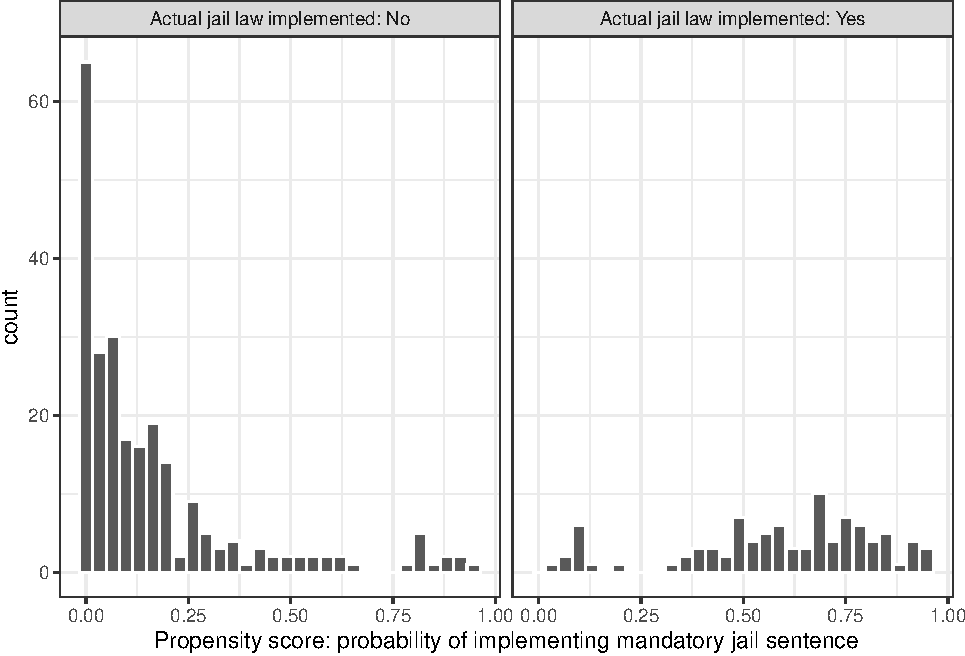
\includegraphics{Project3_Rongkui_files/figure-latex/unnamed-chunk-15-1.pdf}

\emph{Figure Y}: Propensity score distribution across two treatment groups

\begin{Shaded}
\begin{Highlighting}[]
\NormalTok{prs_df }\OperatorTok
\StringTok{  }\KeywordTok{mutate}\NormalTok{(}\DataTypeTok{jail =} \KeywordTok{ifelse}\NormalTok{(jail }\OperatorTok{==}\StringTok{ }\DecValTok{1}\NormalTok{, labs[}\DecValTok{1}\NormalTok{], labs[}\DecValTok{2}\NormalTok{])) }\OperatorTok
\StringTok{  }\KeywordTok{ggplot}\NormalTok{(}\KeywordTok{aes}\NormalTok{(}\DataTypeTok{x =}\NormalTok{ pr_score)) }\OperatorTok{+}
\StringTok{  }\KeywordTok{geom_histogram}\NormalTok{(}\DataTypeTok{color =} \StringTok{"white"}\NormalTok{, }\DataTypeTok{bins =} \DecValTok{30}\NormalTok{) }\OperatorTok{+}
\StringTok{  }\KeywordTok{facet_wrap}\NormalTok{(}\OperatorTok{~}\NormalTok{jail) }\OperatorTok{+}
\StringTok{  }\KeywordTok{xlab}\NormalTok{(}\StringTok{"Propensity score: probability of implementing mandatory jail sentence"}\NormalTok{) }\OperatorTok{+}
\StringTok{  }\KeywordTok{theme_bw}\NormalTok{()}
\end{Highlighting}
\end{Shaded}

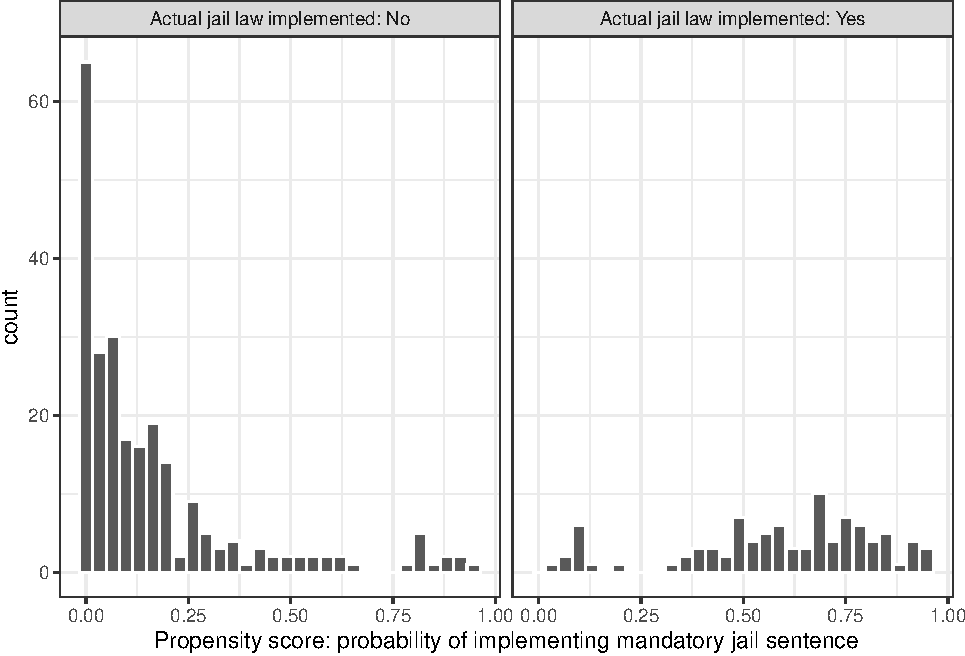
\includegraphics{Project3_Rongkui_files/figure-latex/unnamed-chunk-16-1.pdf}

\hypertarget{matching-1}{%
\subparagraph{3.2.2 Matching}\label{matching-1}}

Nearest neighbor matching algorithm resulted in a new dataset of 188 entires, with 94 original entries with mandatory jail sentence matched with their respective non-treated entry with the most similar propensity score.

\hypertarget{examining-covariate-balance-in-the-matched-sample-2}{%
\subparagraph{3.2.3 Examining covariate balance in the matched sample}\label{examining-covariate-balance-in-the-matched-sample-2}}

\hypertarget{estimate-treatment-effect-1}{%
\subparagraph{3.2.4 Estimate Treatment Effect}\label{estimate-treatment-effect-1}}

\hypertarget{model-diagnostics-1}{%
\paragraph{3.3 Model Diagnostics}\label{model-diagnostics-1}}

\hypertarget{goodness-of-fit-of-logistic-regression-model}{%
\subparagraph{3.3.1 Goodness-of-fit of logistic regression model}\label{goodness-of-fit-of-logistic-regression-model}}

Unlike linear regression with ordinary least squares estimation, there is no \(R^2\) statistic which explains the proportion of variance in the dependent variable that is explained by the predictors. The most notable pseudo \(R^2\) metric commonly used for assessing goodness-of-fit in logistic regression is McFadden's \(R^2\), which is defined as \(1−\frac{log(L_M)}{log(L_0)}\) where \(log(L_M)\) is the log likelihood value for the fitted model and \(log(L_0)\) is the log likelihood for the null model with only an intercept as a predictor. The propensity-score-generating logistic regression model used in this study has a McFadden's \(R^2\) of 0.39, indicating effective removal of a large portion of confounded samples through the propensity score matching process.

\hypertarget{mixed-effect-model}{%
\subparagraph{3.3.2 Mixed Effect model}\label{mixed-effect-model}}

\hypertarget{discussion}{%
\subsection{4.0 Discussion}\label{discussion}}

\hypertarget{propensity-score-matching}{%
\subsubsection{Propensity Score Matching}\label{propensity-score-matching}}

In this report, we highlight the usage of propensity score matching for isolating average treatment effect of implementing mandatory jail sentence upon initial conviction of driving under influence. Rosenbaum and Rubin (1983) defined treatment assignment to be strongly ignorable if the following two conditions hold: (a) treatment assignment is independent of the potential outcomes conditional on the observed baseline covariates, and (b) every subject has a nonzero probability to receive either treatment. They demonstrated that if treatment assignment is strongly ignorable, conditioning on the propensity score allows one to obtain unbiased estimates of average treatment effects. We achieved these conditions through propensity score matching.

\hypertarget{causal-inference}{%
\subsubsection{Causal Inference}\label{causal-inference}}

We cannot confidently draw causal conclusions using the result from this analysis. This is because of the violation of these assumptions necessary for causal inference:

\begin{enumerate}
\def\labelenumi{\arabic{enumi}.}
\item
  The stable unit treatment value assumption (SUTVA):\\
  SUTVA states that the treatment assignment of one experimental unit cannot interfere with the outcome of a separate experimental unit. This is violated in this dataset because\\
\item
  temporal correlations across records taken from the same State, and
\item
  spacial correlations among states that are geographically close to each other.\\
  The implementation of mandatory jail sentence in one state is very likely to influence the vehicle fatality of an adjacent state. And the historic state of the legislation is very likely to influence the vehicle fatality of the same state in the years to come.
\item
  Exogeneity:
  The exogeneity assumption states that the independent variable (implementation of mandatory jail sentence) cannot be dependent on the dependent variable (vehicle fatality rate). This assumption is likely to be violated in this dataset because legislations can arise from existing conditions (\emph{Figure Za}).
\item
  Ignorabilty of unobserved potential confounding variables:
  Although this expansive dataset captures many prominent variables that are associated with vehicle fatality rate, many more economic and social factors come into play in impacting the interactions between the implementation of mandatory jail sentence and vehicle fatality rate. We cannot confidently exclude the possiblity of the existence of many of such variables (\emph{Figure Zb}).
\end{enumerate}

\emph{Figure Z: directed acyclic graphs of scenarios where direction of causal inference changes. a. Violation of exogeneity. b. Violation of ignorability of unobserved confounding variables. M: mandatory jail sentence; F: vehicle fatality rate; UC: unobserved confounding variable}

\begin{Shaded}
\begin{Highlighting}[]
\NormalTok{dag1 =}\StringTok{ }\KeywordTok{dagitty}\NormalTok{(}\StringTok{"dag\{ F -> M \}"}\NormalTok{)}
\NormalTok{dag2=}\StringTok{ }\KeywordTok{dagitty}\NormalTok{(}\StringTok{"dag\{ M <- UC -> F \}"}\NormalTok{)}
\KeywordTok{grid.arrange}\NormalTok{(}\KeywordTok{ggdag}\NormalTok{(dag1), }\KeywordTok{ggdag}\NormalTok{(dag2), }\DataTypeTok{nrow =} \DecValTok{1}\NormalTok{)}
\end{Highlighting}
\end{Shaded}

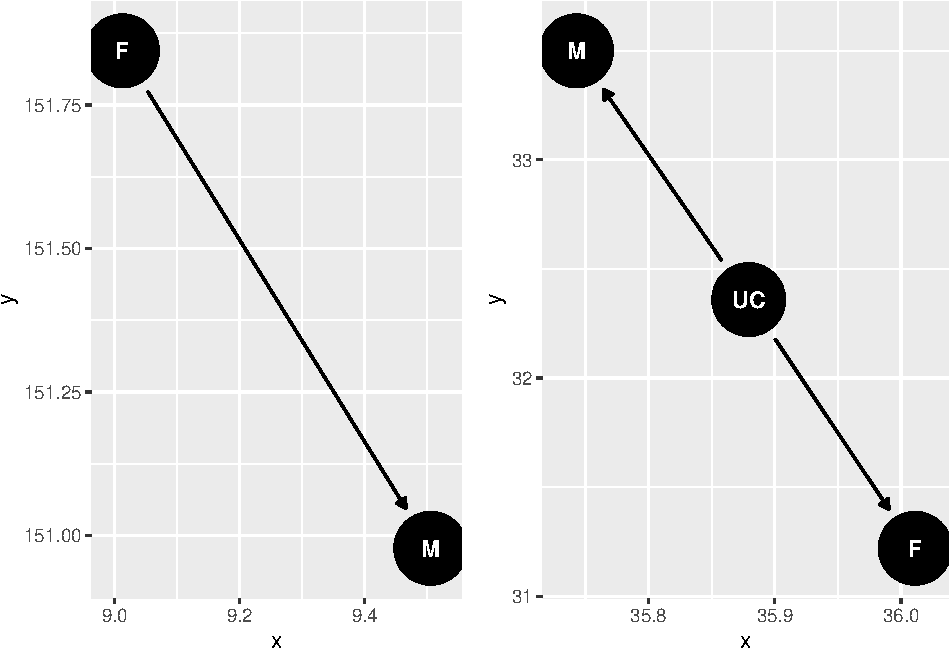
\includegraphics{Project3_Rongkui_files/figure-latex/unnamed-chunk-17-1.pdf}

\hypertarget{reference}{%
\subsection{5.0 Reference}\label{reference}}

Austin P. C. (2011). An Introduction to Propensity Score Methods for Reducing the Effects of Confounding in Observational Studies. Multivariate behavioral research, 46(3), 399--424. \url{doi:10.1080/00273171.2011.568786}\\
Brookhart M.A., Schneeweiss S., Rothman K.J., Glynn R.J., Avorn J., Stürmer T. (2006). Variable selection for propensity score models. American Journal of Epidemiology. 163, 1149--1156.\\
Rosenbaum P.R., Rubin D.B. (1983). The central role of the propensity score in observational studies for causal effects. Biometrika. 70:41--55.
Smith, H. L. (1997). 6. Matching with Multiple Controls to Estimate Treatment Effects in Observational Studies. Sociological methodology, 27(1), 325-353.

\end{document}
